\documentclass[12pt]{article}
\usepackage[french]{babel}
\usepackage{natbib}
\usepackage{url}
\usepackage[utf8x]{inputenc}
\usepackage{amsmath}
\usepackage{graphicx}
\usepackage[svgnames]{xcolor}
\usepackage{vmargin}
\setmarginsrb{3 cm}{1 cm}{3 cm}{1.5 cm}{1 cm}{0.5 cm}{1 cm}{1.5 cm}
\usepackage{multirow}
\graphicspath{{images/}}
\usepackage{parskip}
\usepackage{fancyhdr}
\usepackage[T1]{fontenc}
\usepackage{url}
\usepackage{pdfpages}
\usepackage{url}
\usepackage{hyperref}
\usepackage{graphicx}
\usepackage{subfigure}
\usepackage{caption}
\usepackage{subcaption}
\usepackage{empheq, cases}
\usepackage{amssymb}
\usepackage{amsmath}
\usepackage{verbatimbox}
\usepackage{tcolorbox}
\usepackage{float}
\usepackage{multicol}
\usepackage[compact]{titlesec}
\usepackage[colorinlistoftodos]{todonotes}
\usepackage{sectsty}

\xdefinecolor{gray}{named}{lightgray}
\xdefinecolor{alice}{named}{AliceBlue}
\xdefinecolor{saumon}{named}{PeachPuff}
\definecolor{myred1}{RGB}{255, 0, 0}
\definecolor{mygreen1}{RGB}{0, 126, 0}
\definecolor{myblue1}{RGB}{0, 0, 61}
\definecolor{lightgray}{rgb}{0.83, 0.83, 0.83}
\definecolor{brick}{rgb}{0, 0, 0.50}
\sectionfont{\color{brick}}  % sets colour of chapters
\subsectionfont{\color{RoyalBlue}}

\tcbset{colback=lightgray,colframe=black}



\title{\color{brick} Optimisation TD 4:\\
\LARGE{Recuit simulé et le voyageur de commerce}}								% Title
\author{Émilie Mathian}								% Author
\date{Année 2018 - 2019}											% Date

\makeatletter
\let\thetitle\@title
\let\theauthor\@author
\let\thedate\@date
\makeatother

\pagestyle{fancy}
\fancyhf{}
\rhead{\theauthor}
\lhead{Optimisation TD 1}
\cfoot{\thepage}
%%%%%%%%%%%%%%%%%%%%%%%%%%%%%%%%%%%%%%%%%%%%%%%%%%%%%%%%%%%%%%%
\usepackage{eso-pic}
\newcommand\BackgroundPic{%
\put(0,0){%
\parbox[b][\paperheight]{\paperwidth}{%
\vfill
\centering
\includegraphics[width=\paperwidth,height=\paperheight,%
keepaspectratio]{background.png}%
\vfill
}}}
  
  
\begin{document}

%%%%%%%%%%%%%%%%%%%%%%%%%%%%%%%%%%%%%%%%%%%%%%%%%%%%%%%%%%%%%%%%%%%%%%%%%%%%%%%%%%%%%%%%%

\begin{titlepage}
	\centering
    \vspace*{0.5 cm}
    \vspace{-3.5cm}
    
\includegraphics[width = 4cm]{logo.png}\\	% University Logo
    \textsc{\LARGE Institut National des Sciences Appliquées de Lyon}\\[2.0 cm]	% University Name
	\textsc{\Large $4^{eme}$ Année Bioinformatique et Modélisation}\\[0.5 cm]				% Course Code
	\textsc{\large Professeur: Noëlie DEBS }\\[0.5 cm]				% Course Name
	\rule{\linewidth}{0.2 mm} \\[0.4 cm]
	{ \huge \bfseries \thetitle}\\
	\rule{\linewidth}{0.2 mm} \\[1.5 cm]
	
	\begin{minipage}{0.4\textwidth}
		\begin{flushleft} \large
			\emph{Auteur:}
			\theauthor
			\end{flushleft}
			\end{minipage}~
			\begin{minipage}{0.4\textwidth}	
	\end{minipage}\\[2 cm]
    \vspace{-1.8cm}
	 \begin{figure}[H]
	\begin{center}
	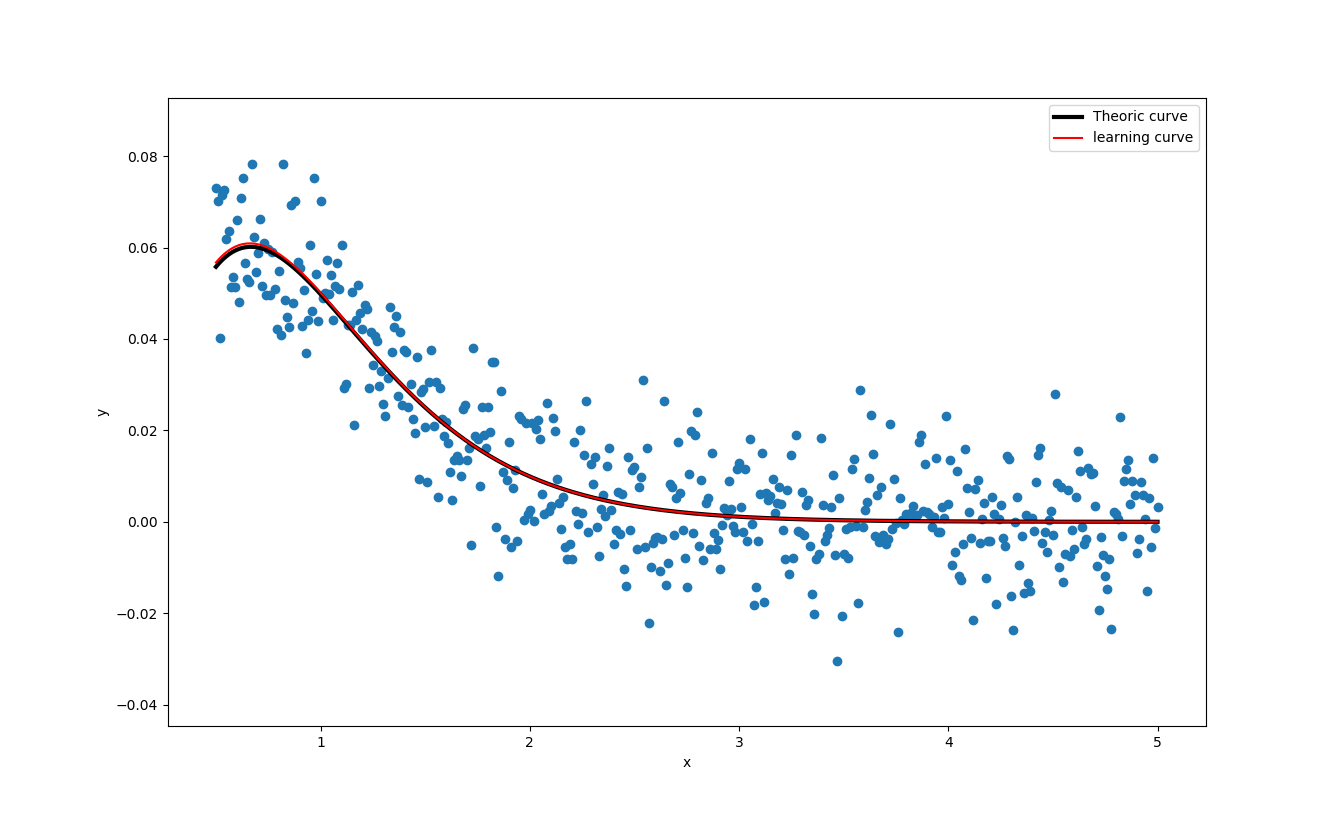
\includegraphics[width=0.9 \textwidth]{Figure_1.png}
\end{center}
\end{figure}

	{\large \thedate}\\[1 cm]
    
	\vfill

 

\end{titlepage}
\pagebreak
%%%%%%%%%%%%%%%%%%%%%%%%%%%%%%%%%%%%%%%%%%%%%%%%%%%%%%%%%%%%%%%%%%%%%%%%%%%%%%%%%%



\newpage 

\tableofcontents

\newpage
\begin{center}
\fcolorbox{black}{lightgray}{
\begin{minipage}{\linewidth}
\textbf{Problématique :} \\
Le recuit simulé est un algorithme d'optimisation intégrant une part d'aléatoire. Cet algorithme est une analogie à une technique employée en métallurgie, où la fonction à minimiser est l'énergie libre d'un métal. Par comparaison à la thermodynamique,  la probabilité de trouver un système d'énergie $E_S$ est fonction de la température tel que $p(X=E_S) = e^{-E_s/T}$ (probabilité de Boltzmann), alors on peut considérer que la probabilité d'avoir atteint le minimum local d'une fonction est fonction d'une fonction décrivant l'évolution de la température et de la connaissance du voisinage de la solution courante .

Nous observerons l'importance de cette loi qui donne de la souplesse à l'algorithme. Nous mettrons aussi en évidence l'importance de la recherche locale du minimum global et l'importance du périmètre de recherche. De plus par comparaison à la métallurgie où  On voudrait ainsi obtenir un métal ayant la plus grande stabilité soit un cristal, on sait cet état n'est atteint que lorsque le processus de refroidissement est lents, sinon on risque d'obtenir un polycristal de plus haute énergie libre, ainsi la recherche du minimum global est efficace lorsque le paramètre T décroît lentement, c'est à dire quand on augmente lentement la probabilité d'accepter de mauvaises solutions et qu'on accroît doucement le périmètre de recherche. Nous étudierons  ainsi l'effet du  schéma du refroidissement. \\
Le rapport suivant reprend le programme \textit{'recuit.py'}, certains résultats ont été repris avec le script \textit{Results_TD4.rmd}.
\end{minipage}}
\end{center} 

\section{Le recuit simulé}



\subsection{Fonction de $\mathbb{R}$ dans $\mathbb{R}$}
\begin{minipage}{0.5\textwidth}

\textbf{\color{brick}1.} 
D'après la représentation de la fonction $f(x)$ \textbf{[\ref{Q1}]}, nous observons l'existence d'un minimum local et d'un minimum global. Nous pouvons numériquement estimer les coordonnées de ces points d'inflexion. Le minimum local est atteint pour $x\simeq 2.823$ alors $f(2.823)\simeq -114.55$, le maximum local est atteint pour $x\simeq0.024$ alors $f(0.024)\simeq 1.012$ et enfin le minimum global est atteitn pout $x\simeq 3.548$ et alors $f(3.548)\simeq -133.41$.
\end{minipage} \hfill
\begin{minipage}{0.45\textwidth}
\begin{figure}[H]
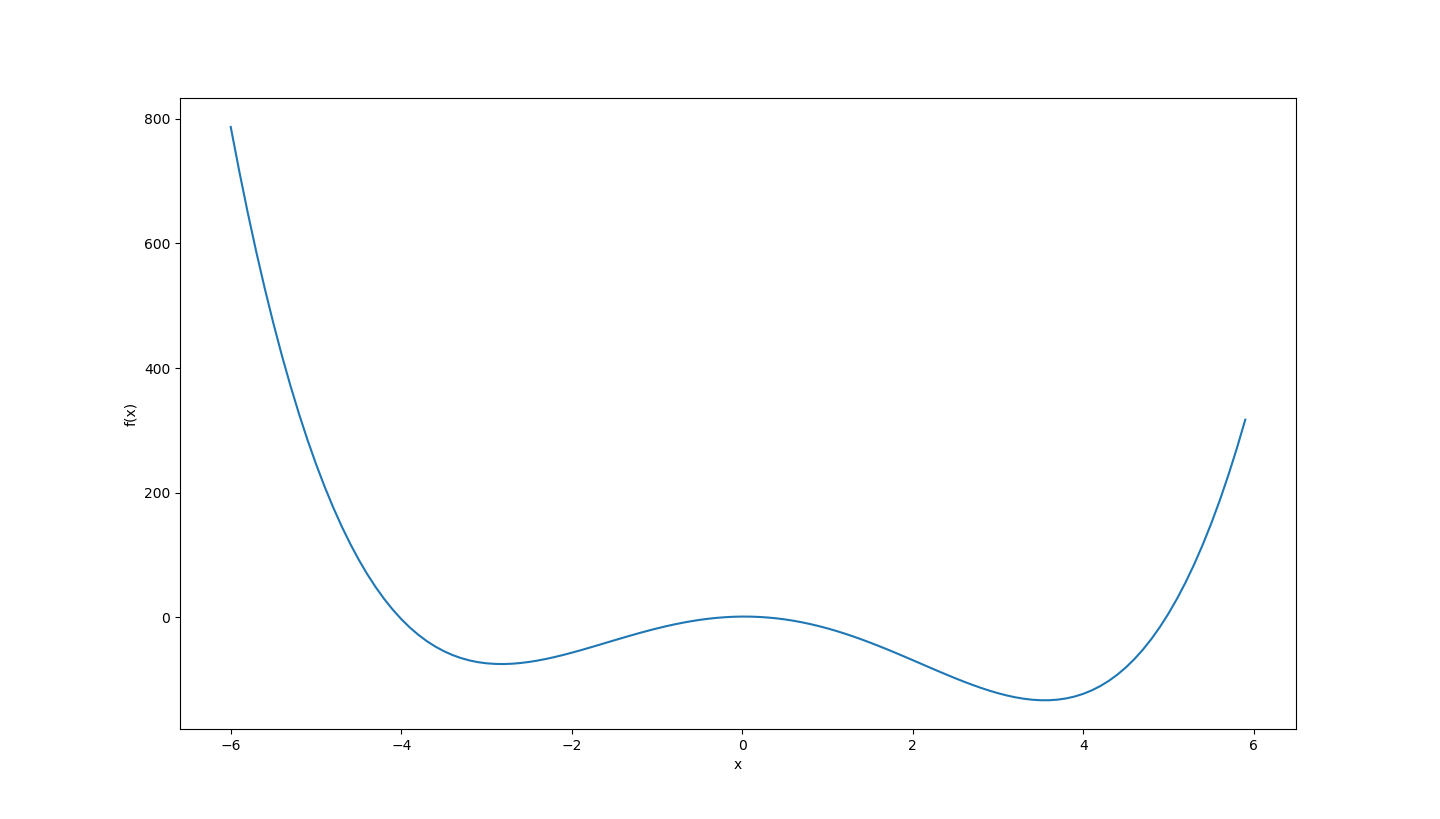
\includegraphics[width=1\textwidth]{Q1.png}
\caption{Représentation de la fonction à minimiser  $f(x)=x^4 - x^3 -20x^2+x+1$}
\label{Q1}
\end{figure}
\end{minipage}


\begin{minipage}{0.5\textwidth}
\textbf{\color{brick}2.} L'implémentation de la méthode du recuit simulé pour la fonction $f$  fait référence à la fonction \verb|recuit_f1| (cf : \verb|recuit.py|).\\
 Pour tester notre algorithme nous prenons les conditions suivantes : $k=10$, $k'=0.5$, $T=1/t$ et $t_{max}=1$, la solution obtenue est illustrée ci-contre \textbf{[\ref{Q1_2}]}. Nous remarquons que la solution converge vers le minimum global, avec comme résultat final $x_{t=10000} \simeq 3.548  $ et $f(x_{t=10000}) \simeq -133.41$. En revanche l'algorithme a parcouru un vaste espace vers des valeurs très éloignées de la solution avant de converger.
\end{minipage} \hfill
\begin{minipage}{0.45\textwidth}
\begin{figure}[H]
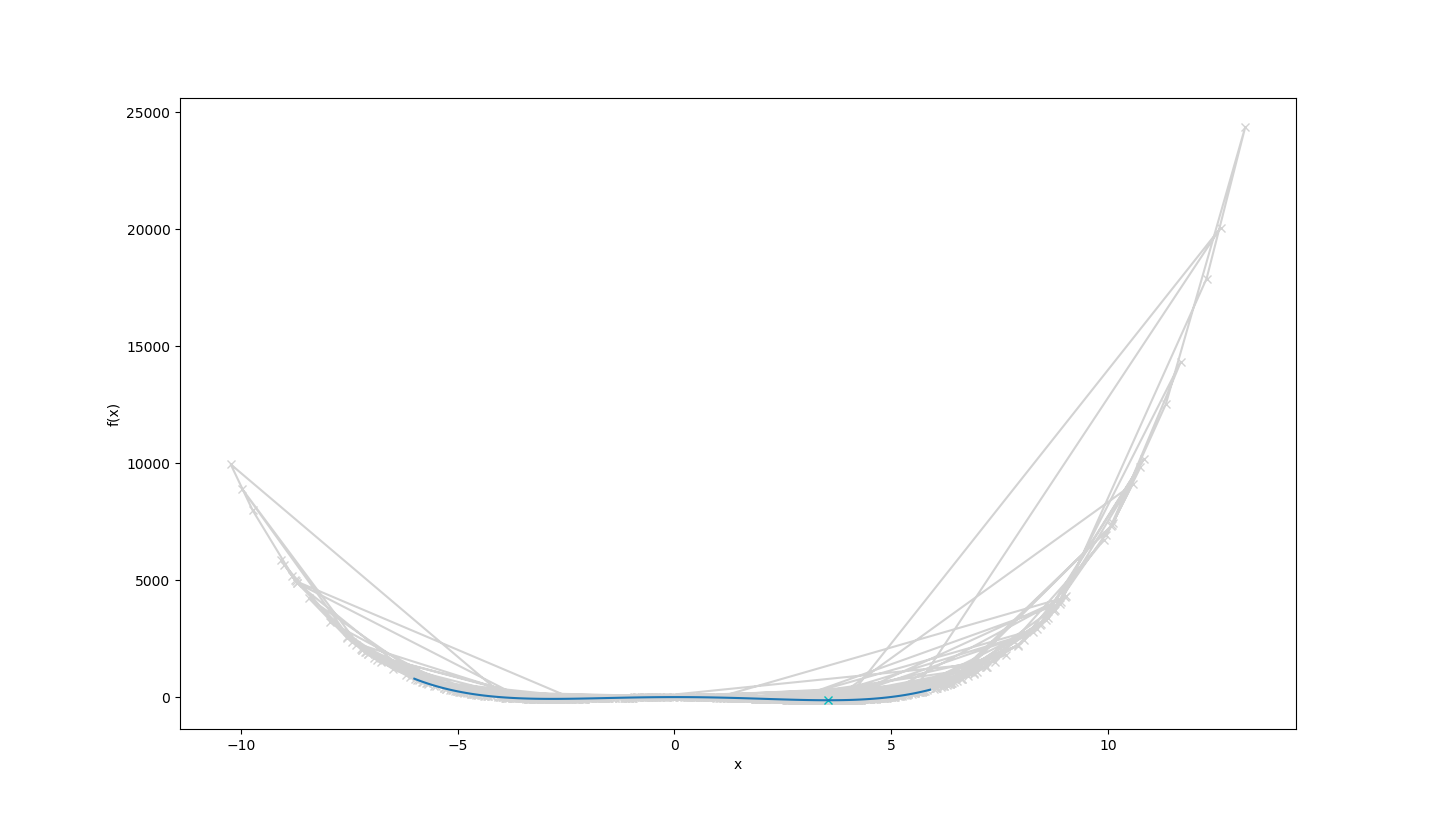
\includegraphics[width=1\textwidth]{Q1_2.png}
\caption{Représentation de la fonction à minimiser  $f$, du parcours de l'algorithme du recuit simulé et de la solution finale retenue.}
\label{Q1_2}
\end{figure}
\end{minipage}

\begin{figure}[H]
  \centering
  \subfigure[Variation de k]{%
    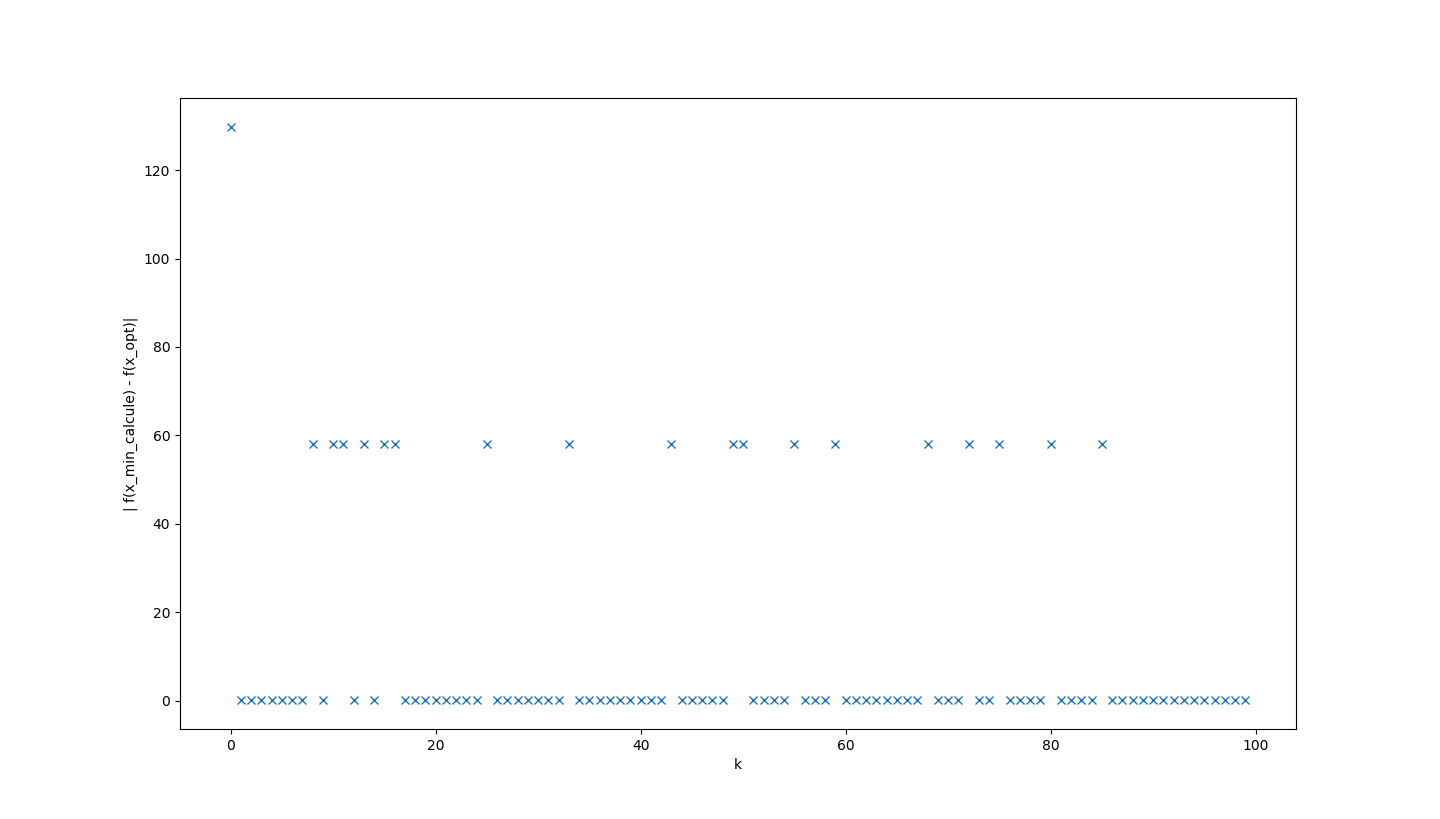
\includegraphics[width=0.45\textwidth]{Q1_k.png}
    \label{fig:a}%
    }%or more
    \subfigure[Variation de k']{%
    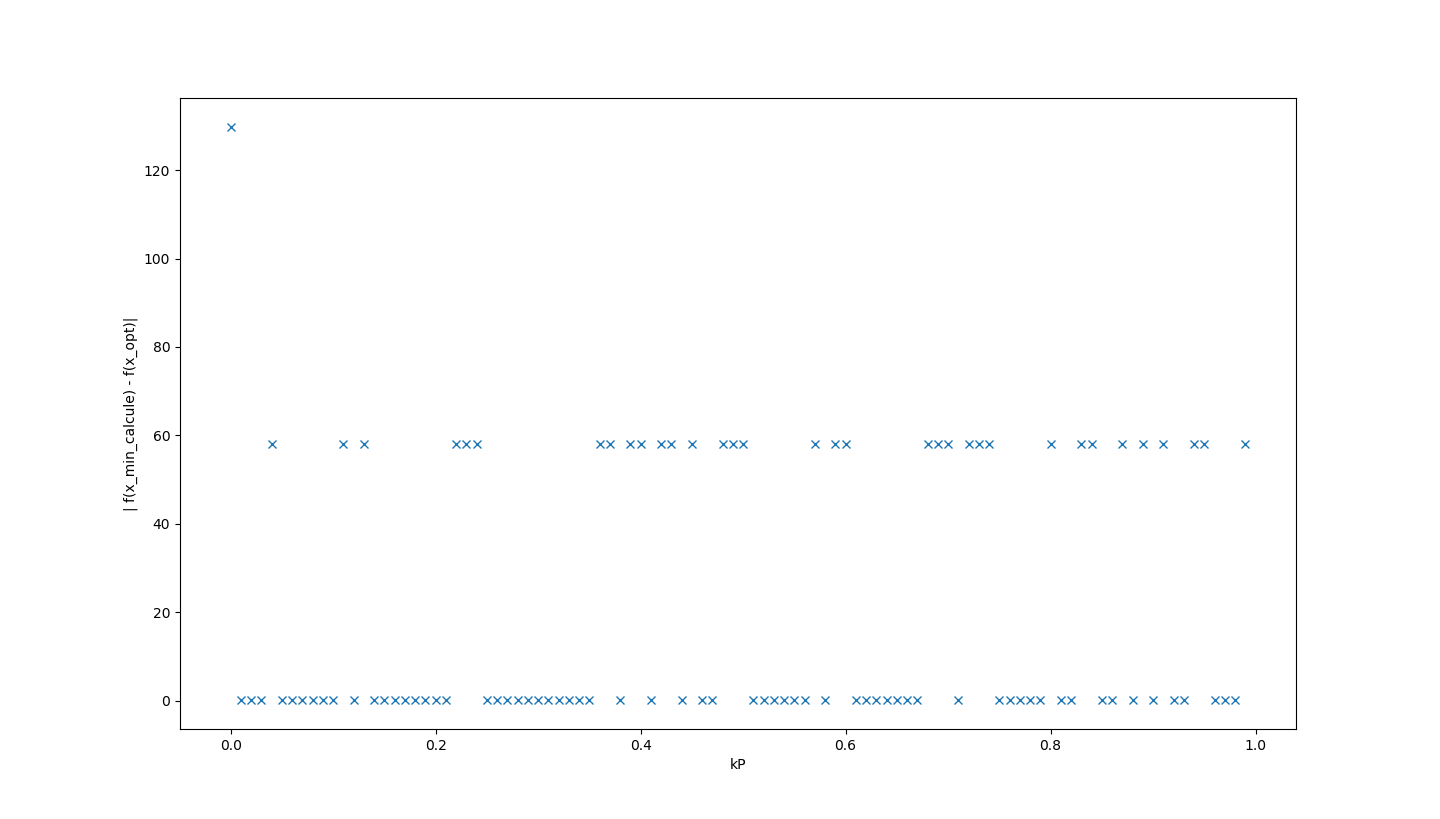
\includegraphics[width=0.45\textwidth]{Q1_kp.png}
    \label{fig:b}%
  }%  
  \caption{Représentation de l'écart entre la solution calculée et la solution analytique pour 10000 itération avec $x_0 = 0.5$, et pour \textbf{a} $kp=0.5$ et $k\in [0,15]$ et  pour \textbf{b} $kp \in [0,1]$ et $k= 10$}
  \label{fig:ab}
\end{figure}
D'après la figure \textbf{[\ref{fig:a}]}, on observe que l'algorithme converge plus fréquemment vers le minimum global lorsque k est grand, la densité du nuage de point, est plus forte à droite. Ainsi plus on permet à l'algorithme d'inspecter un voisinage éloigné du $x$ courant plus  la probabilité de trouver le minimum global croit. En augmentant$k$ on autorise, particulièrement en fin du processus, la recherche de solutions dans un voisinage de plus en plus grand  ce qui permettrait schématiquement de  s'échapper d'un minimum local en testant des solutions incongrues.\\ 
 À l'inverse d'après la figure \textbf{[\ref{fig:b}]} plus $k'$ diminue (noté kp)  plus la probabilité de converger vers le minimum global augmente, la densité du nuage de point est plus forte à droite. Ainsi plus on abaisse la probabilité d'accepter un point qui augmentait localement le coût plus la probabilité de converger vers le minimum global croît.\\
 Soulignons cependant que le choix des paramètres est un compromis entre le temps de calcul et l'éfficacité (convergence vers le minimum global).\\
 Néanmoins ces remarques semblent approximatives et pourraient être dues au hasard.\\
 
 %%%%% Mettre en évidence cette vitesse de convergent
 
C'est pourquoi nous allons tenter de mettre en place une procédure statistique pour savoir si le nombre de succès est fonction des paramètres $k$ ou $kp$. Pour cela nous choisissons de séparer les valeurs du paramètre  testées en quatre classe et de tester hypothèse suivantes, où $S$ représente le nombre de succès :
\begin{align*}
    H_O : \quad S_{k=m1} &=  S_{k=m2} &=  S_{k=m3} =S_{k=m4}  \\
    H_1 : \quad Au moins une des condition est différente
\end{align*}

Pour réaliser ce test nous générons 40 échantillons contenant chacun une répétition pour chaque valeur du paramètre. Nous obtenons donc 40 vecteurs binaires où $1$ représente un succès. Nous sommons le nombre de succès pour chaque simulations en fonction des différentes valeurs prise par le paramètre, $k$ ou $kp$.  Nous exportons les vecteurs dans R. Puis nous regroupons les données  par classe.   Nous réalisons alors un test de Bartlett pour vérifier l'homoscédasticité. Si celle-ci est vérifier nous réalisons un test de Kruskall Wallis (cf : Hypothèse ci-dessus). Si le test de Kruskal Wallis nous permet de rejeter $H_0$ au seuil $\alpha=5\%$ alors nous effectuons des test multiples grâce à la procédure de Nemenyi.\\
Remarquons enfin que les fonctions tels qu'elles sont écrites dans le script \verb|recuit.py|, permettent de choisir aléatoirement une condition initiale, nous utiliserons cette propriété  pour  les simulations.\\ 
\begin{minipage}{0.5\textwidth}

\textbf{\color{brick}1.} 
L'homoscédasticité des variances est vérifiée (p_value de Bartlett.test = 0.6). Le test de Kruskall wallis avec une $p-value = 0.39$ permet de rejeter H0, ainsi au risque $\alpha=5\%$ nous rejetons le fait que les médianes par ckasse sont identiques. Le test de Nemenyi permet de mettre en évidence que les deux classes testées statistiquement différentes sont $k\in(7.25,11]$et  $k\in(0,3.5]$ (cf: Results\_R.rmd partie 1.1). Ainsi il semble y avoir une valeur optimale de k, permettant d'augmenter le nombre de succès 
\end{minipage} \hfill
\begin{minipage}{0.45\textwidth}
\begin{figure}[H]
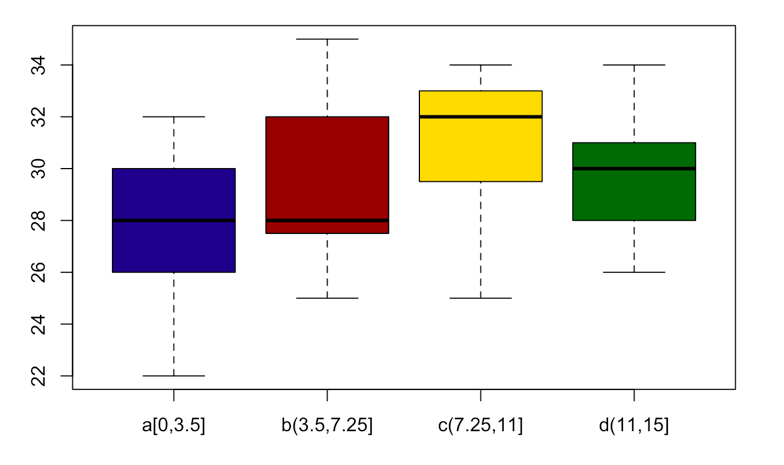
\includegraphics[width=1\textwidth]{nombre_succes-K_F.png}
\caption{Représentation de la simulation décrite précédemment en fixant $t_max=10000$, $k'=0.5$ et en faisant varier le paramètre $k$ entre $[0,15]$, nous prenons un pas de 0.25 (50 valeurs de $k$ sont ainsi testées). Nous regroupons nos résultats en quatre classes.}
\label{nombreSkf}
\end{figure}
\end{minipage}


Ces conclusions sont vrais si on s'interesse sur l'intervalle $k'\in[0,05]$, en effet si on réalise ce test sur $[0,1]$ la différence de moyennes n'est plus significatives !

\begin{minipage}{0.5\textwidth}
L'homoscédasticité est vérifiée, le test de Kruskall wallis permet de rejeter H0. Le test de Nemenyi permet de mettre en évidence que les classe $k' \in(0,0.22 ] $ et $k'\in (0.72,1]$ sont significativement différente. Ainsi comme nous pouvons l'observer graphiquement le nombre de succès est plus grand lorsque $k'$ diminue mais on peut également observer la variabilité de la classe 'a' même si celle si n'est pas significative. (cf : Results\_R.rmd partie 1.2)
\end{minipage} \hfill
\begin{minipage}{0.45\textwidth}
\begin{figure}[H]
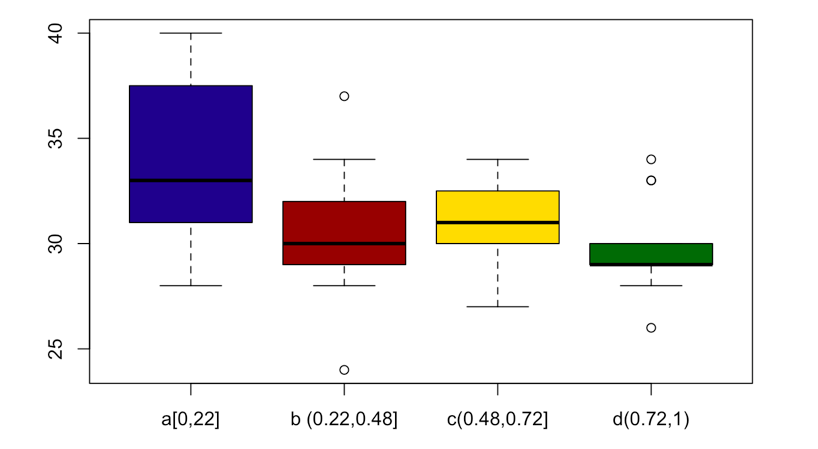
\includegraphics[width=1\textwidth]{NombreSuccesKp_F.png}
\caption{Représentation de la simulation décrite précédemment en fixant $t_max=10000$, $k=10$ et en faisant varier le paramètre $k'$ entre $[0,1]$, nous prenons un pas de 0.02 (60 valeurs de $k$ sont ainsi testées). }
\label{nbSkpF}
\end{figure}
\end{minipage}



\begin{minipage}{0.5\textwidth}
Rappelons que le choix du nombre d'itérations maximale influence également la température étant donnée que $T=\frac{1}{t}$, pour observer l'influence de la température nous pouvons faire varier le coefficient  '1000' pour ralentir ou augmenter le processus de refroidissement. Nous faisons donc varier ce coefficient entre $[0,2000]$ et nous obtenons les résultats ...
% Ref image
\end{minipage} \hfill
\begin{minipage}{0.45\textwidth}
\begin{figure}[H]
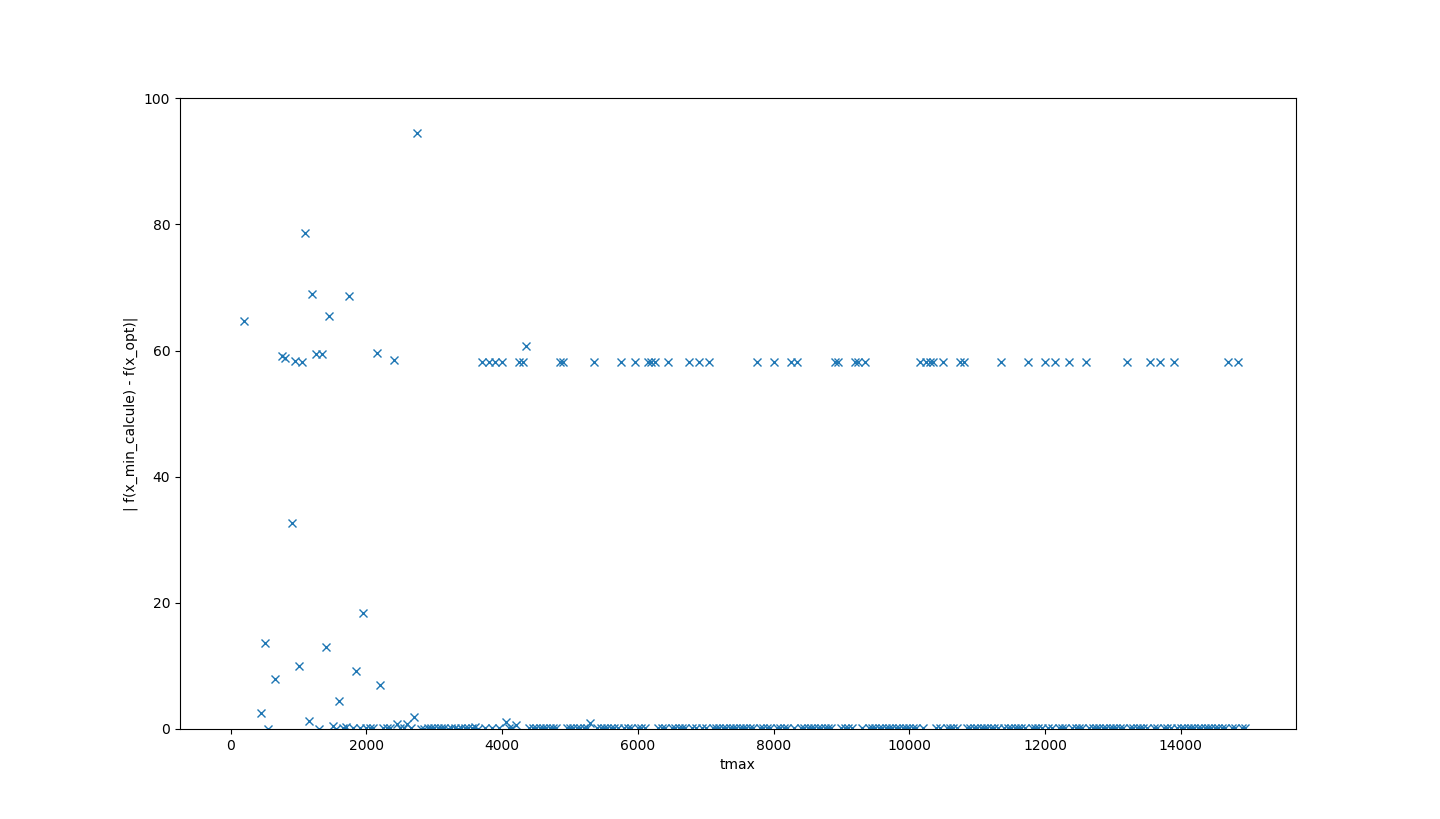
\includegraphics[width=1\textwidth]{Q1_T.png}
\caption{valeur absolue de l'erreur en fonction du nombre d'itération maximal}
\label{Q1_T}
\end{figure}
\end{minipage}

\textbf{\color{brick}3.} D'après les analyses précédentes pour augmenter la convergence de l'algorithme vers le minimum global nous choisissons $k=20$, $k'p=0.1$ et $t_{max}=15000$, nous obtenons alors les résultats suivants:
\begin{figure}[H]
\centering
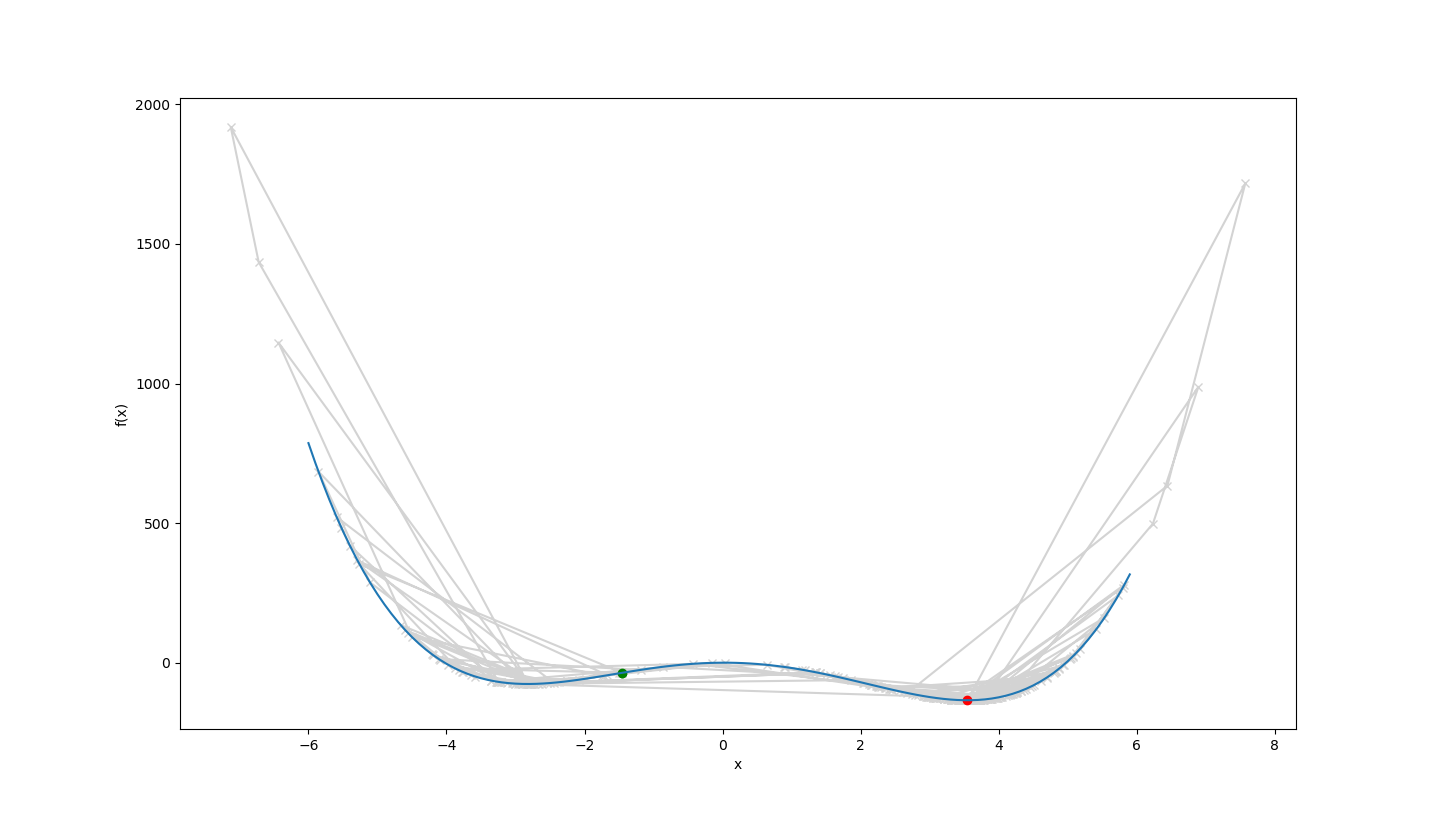
\includegraphics[width=0.7\textwidth]{Q132.png}
\caption{Représentation de l'évolution de l'algorithme (gris), à la surface de $f$ (bleu), le point de départ est indiqué en vert et celui d'arrivée en rouge.}
\label{Q1_T}
\end{figure}

\begin{center}
\fcolorbox{black}{lightgray}{
\begin{minipage}{\linewidth}
\textbf{Remarque sur l'algorithme :} \\
\begin{itemize}
    \item Le point de départ est choisi aléatoirement dans une lois uniforme selon deux bornes données par l'utilisateur.
    \item En plus du critère d'arrêt établi par rapport à un nombre d'itérations, une seconde condition d'arrêt a été établi sur le pourcentage d'acceptation, c'est à dire le nombre de mouvement retenu par rapport au nombre d'itérations total. On peut en effet estimer que si ce pourcentage est faible alors l'algorithme ne conserve que très rarement des solutions, et est donc dans un minimum local de la fonction de coût.\\
    
\end{itemize}
\end{minipage}}
\end{center}

\subsection{Fonction de $\mathbb{R}^2$ dans $\mathbb{R}$}
Nous étudions la fonction $g(x,y)= x^4-x^3-20x^2+x+1 +y^4-y^3-20y^2+y+1$; cette fonction a été dans le TD 1 exercice 3; ainsi nous savons qu'elle possède 9 points caractéristique, un maximum local, quatre points selle , et 4 minimum dont un minimum global \textbf{[\ref{Q21}}.
\begin{figure}[H]
\centering
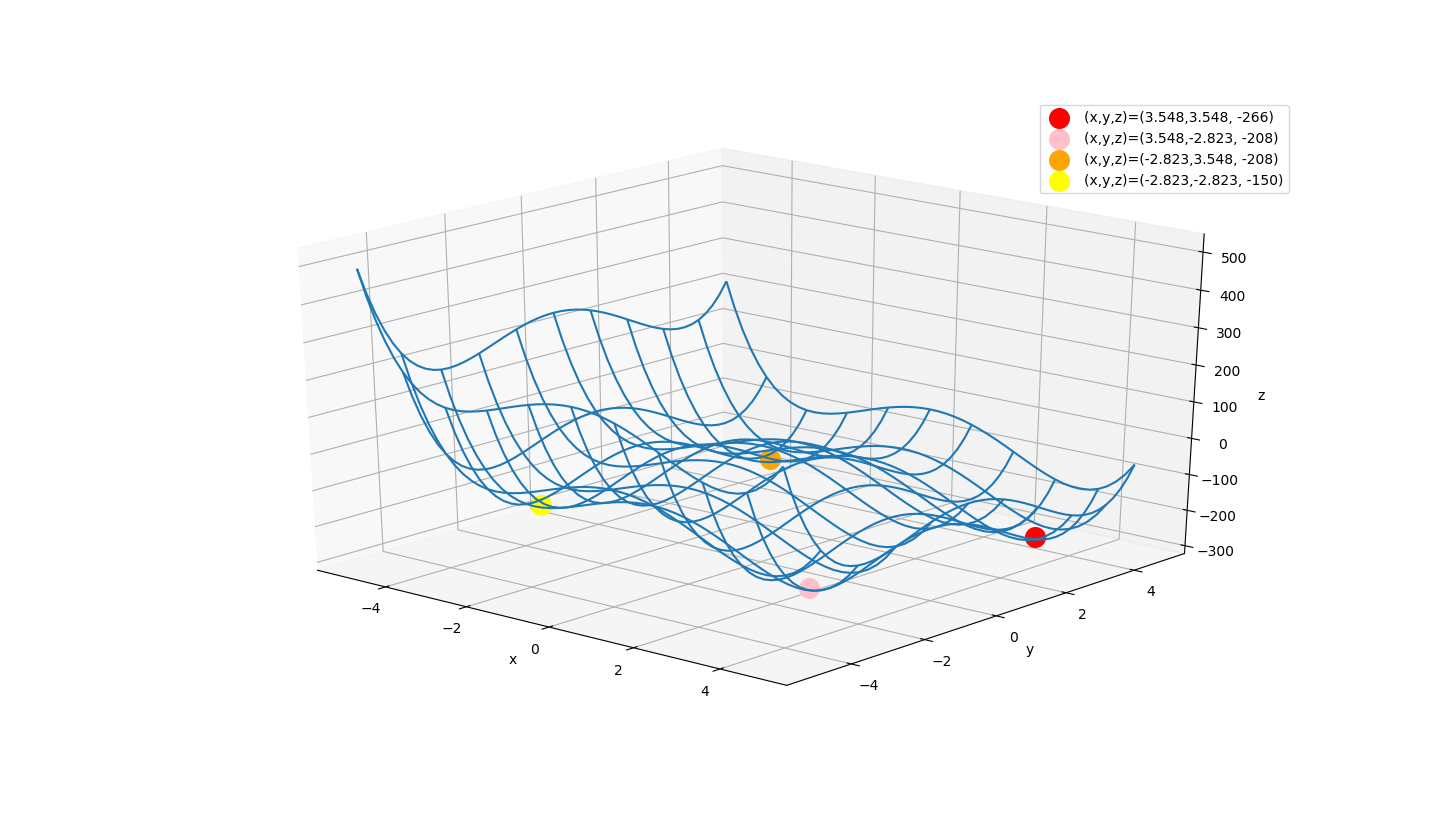
\includegraphics[width=0.7\textwidth]{Q21.png}
\caption{Représentation de la fonction g et de ces quatre minimums, et de leurs coordonnées.}
\label{Q21}
\end{figure}

\begin{minipage}{0.5\textwidth}
Nous reprenons l'analyse des paramètres avec la même stratégie que dans le cas précédent ainsi en fixant $k'=0.5$, $x_0=0$, $y_0=0$ et $t_{max}=10000$ nous faisons varier $k$ tel que $k\in [0,30]$ . Graphiquement il est difficile de conclure sur l'influence du paramètre \textbf{[\ref{Q2K}]}
. Il en est de même en faisant varier $k'$ les autres paramètres restant égaux par ailleurs.
\end{minipage} \hfill
\begin{minipage}{0.45\textwidth}
\begin{figure}[H]
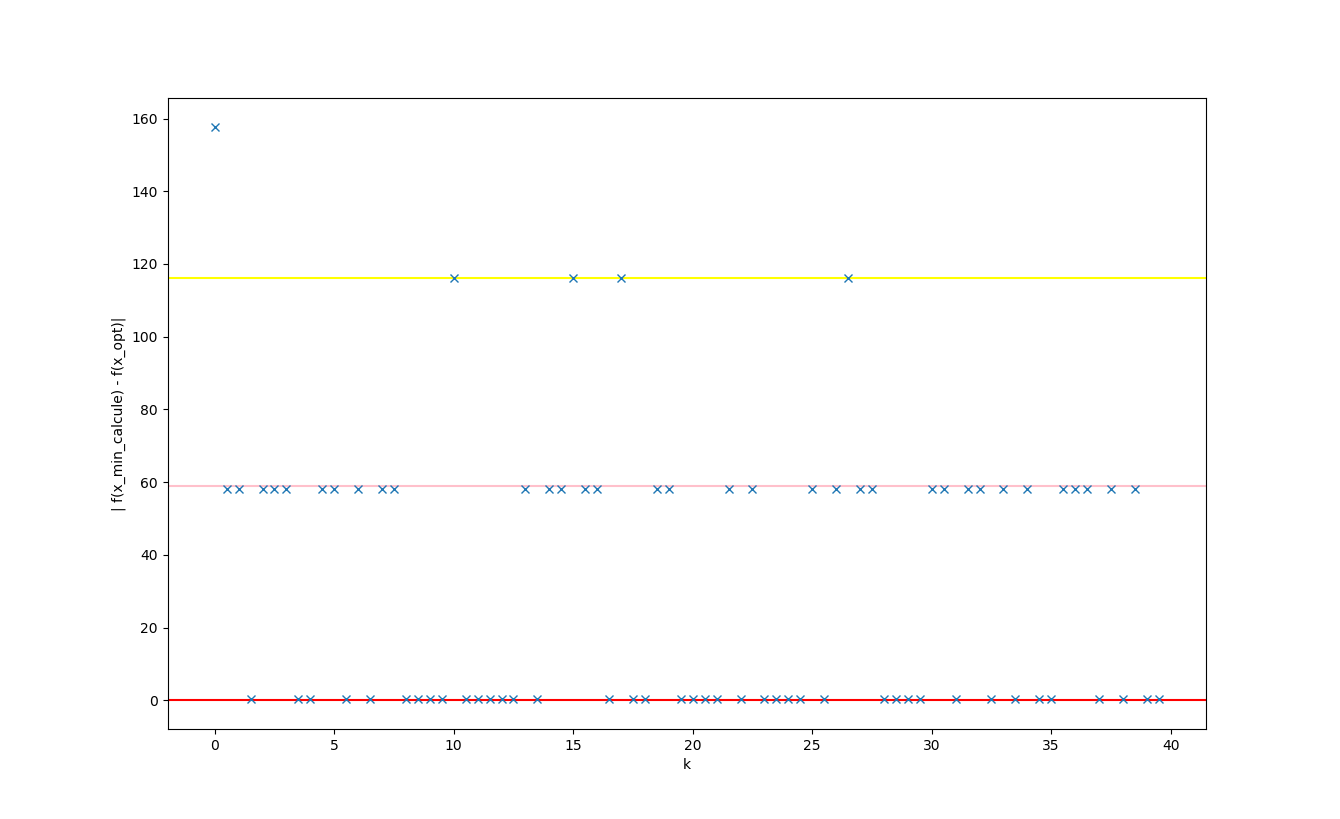
\includegraphics[width=1\textwidth]{Q2K.png}
\caption{Représentation de la fonction g et de ces quatre minimums, et de leurs coordonnées.}
\label{Q2K}
\end{figure}
\end{minipage}
\\
Nous utilisons lea procédure mise en place pour analyser ces résultats :


\begin{minipage}{0.5\textwidth}
 Si les variances sont homogènes d'après le test de Bartlett. Le test de Kruskall Wallis  ne permet pas de distinguer l'un des groupes. En effet on obtient une $p-value = 0.184$, on ne peut pas rejeter $H_0$. Nous pouvons pourtant faire l'hypothèse que le mécanisme est identique que dans le cas précédant étant l'allure des solutions, il se peut que le choix des classes ne permettent cependant pas de mettre en évidence cet effet.
\end{minipage} \hfill
\begin{minipage}{0.45\textwidth}
\begin{figure}[H]
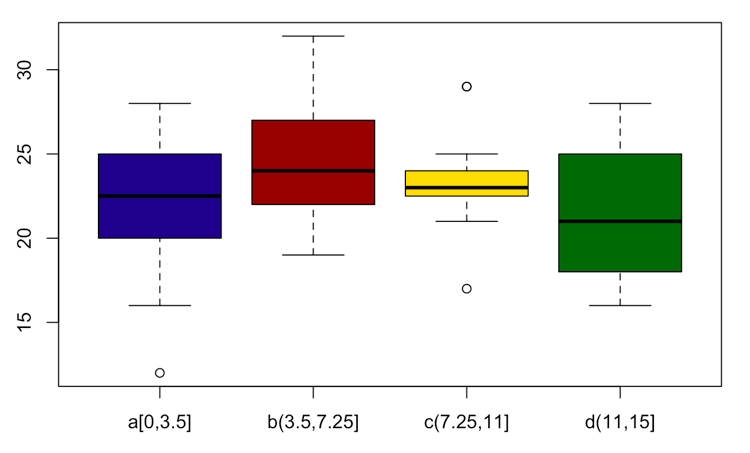
\includegraphics[width=1\textwidth]{nombresucces_k_G.png}
\caption{Représentation de la simulation décrite précédemment en fixant $t_max=10000$, $k'=0.5$ et en faisant varier le paramètre $k$ entre $[0,15]$, nous prenons un pas de 0.25 (50 valeurs de $k$ sont ainsi testées). Nous regroupons nos résultats en quatre classes.}
\label{Q2K}
\end{figure}
\end{minipage}



\begin{minipage}{0.5\textwidth}
 Une fois de plus, si les variances sont homogènes d'après le test de Bartlett. Le test de Kruskall Wallis  ne permet pas de distinguer l'un des groupes. En effet on obtient une $p-value = 0.179$, on ne peut pas rejeter $H_0$. Ainsi même si l'influence de $k'$ est théoriquement identique elle est plus difficilement détectable. Remarquons que le nombre de succès moyen quelque soit la classe de $k'$ ou $k$ est plus faible pour la fonction $g$ que pour la fonction $f$, ceci pourrait s'expliquer par la complexité de cette fonction. On tente d'améliorer l'efficacité de la méthode en fixant $tmax =20000$ , $k=15$, $k' = 0.1$, en effet pour pouvoir tester ces paramètre nous devons faire un compromis sur le temps de calcul. On obtient pour 40 répétions  65\% de succès contre 55\% avec les données du graphique \textbf{[\ref{Q2KP}]}.
\end{minipage} \hfill
\begin{minipage}{0.45\textwidth}
\begin{figure}[H]
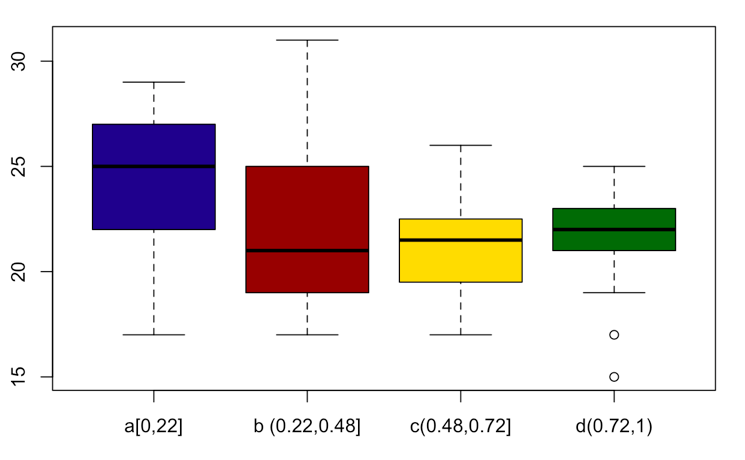
\includegraphics[width=1\textwidth]{nSKPG.png}
\caption{Représentation de la simulation décrite précédemment en fixant $t_max=10000$, $k=10$ et en faisant varier le paramètre $k'$ entre $[0,1]$, nous prenons un pas de 0.02 (60 valeurs de $k$ sont ainsi testées).}
\label{Q2KP}
\end{figure}
\end{minipage}

\subsection{Compréhension de l’algorithme}
\textbf{\color{brick}1.} L'algorithme du recuit simulé explore l'espace de façon aléatoire, ce type de recherche du minimum peut être bénéfique lorsque :
\begin{itemize}
    \item la fonction à minimiser n'est pas dérivable,
    \item la fonction à minimiser n'est pas continue,
    \item l'algorithme 'chute' dans un minimum local, il peut le contourner.
\end{itemize}
\vspace{0.5cm}
\textbf{\color{brick}2.} La température intervient deux fois dans l'algorithme du recuit simulé. Une première fois dans le choix d'un $x$ voisin de la position courante avec $X_{t+1}= x_t + N(0, ke^{-1/1000T})$, et une seconde fois dans la probabilité d'accepter un $x$ induisant une augmentation de la fonction de coût. En début de simulation  $T =1$ le voisinage es définit sur un grand espace et la probabilité d'accepter ce voisin est relativement grande, en fin de simulation $T$ est faible alors la recherche de voisins est réalisée dans une surface petite et la probabilité d'acceptation est faible. \\
Par analogie aux processus de recuit en début de processus le niveau d'énergie du système, auquel peut être associé la fonction de coût, est relativement grand, ce niveau d'énergie fluctue ensuite aléatoirement jusqu'à atteindre d'un équilibre thermique. De plus en physique la loi de Bolltzman nous apprend que la probabilité d'observer un système à une énergie donné $E$ est fonction de la température de l'environnement telle que $e^{-E/T}$, ainsi plus la température diminue plus la probabilité d'observer cet état diminue.  \\
En d'autre terme à l'initiation du processus l'algorithme procède à une recherche 'naïve' sans connaissance de l'environnement énergétique, ainsi l'algorithme progresse  par  oscillations, puis l'ampleur de ces oscillations est diminue avec la température. À la fin du processus les oscillations sont quasi nuls ce qui nous permet de conclure à la convergence de l'algorithme.\\
Cependant la convergence vers un minimum global n'est pas garanti, il dépend d'un compromis entre le temps de calcul et le meilleur résultat possible. En effet si la décroissance thermique est trop rapide l'algorithme perd rapidement en 'souplesse' et risque de converger vers un minimum local.\\
\\
\textbf{\color{brick}3.} Comme nous l'avions expliqué $k'$ permet de pondérer la probabilité d'acceptation de voisins induisant une augmentation de la fonction de coût. Plus on diminue $k'$ plus on restreint l'exploration, on pourrait ainsi  augmenter l'efficacité mais ceci dépend de la condition initiale. En étant laxiste envers l'erreur on augmente l'aire explorée mais là encore  on ne garantit pas la convergence vers un minimum global. Il existe une valeur optimale de $k'$.\\
Le paramètre $k$ pondère l'ampleur des oscillation, à l'instar du paramètre $k'$ une augmentation de $k$ accroît l'aire explorée et donne une certaine souplesse à l'algorithme, réciproquement une diminution de $k$ pourrait augmenter la vitesse de convergence à condition d'être dans le voisinage du minimum global.

\subsection{Modification du schéma de refroidissement}
% penser à  illustrer delta e au cours des itérations 
% évolution de la température 
\textbf{\color{brick}1,2,3.}
Nous modifions l'algorithme de recuit simulé en introduisant un palier de température, ainsi la probabilité de conserver une 'mauvaise' décision sera fonction de la variation locale de la fonction de coût $\Delta E$ au voisinage de la position courante. Cette modification a été implémentée dans les fonction \verb|recuit_f1_p | et \verb|recuit_g_p|.
\textbf{\color{brick}4.}
\textbf{\color{brick}4.}
\begin{figure}[H]
  \centering
  \subfigure[cas de la fonction f]{%
    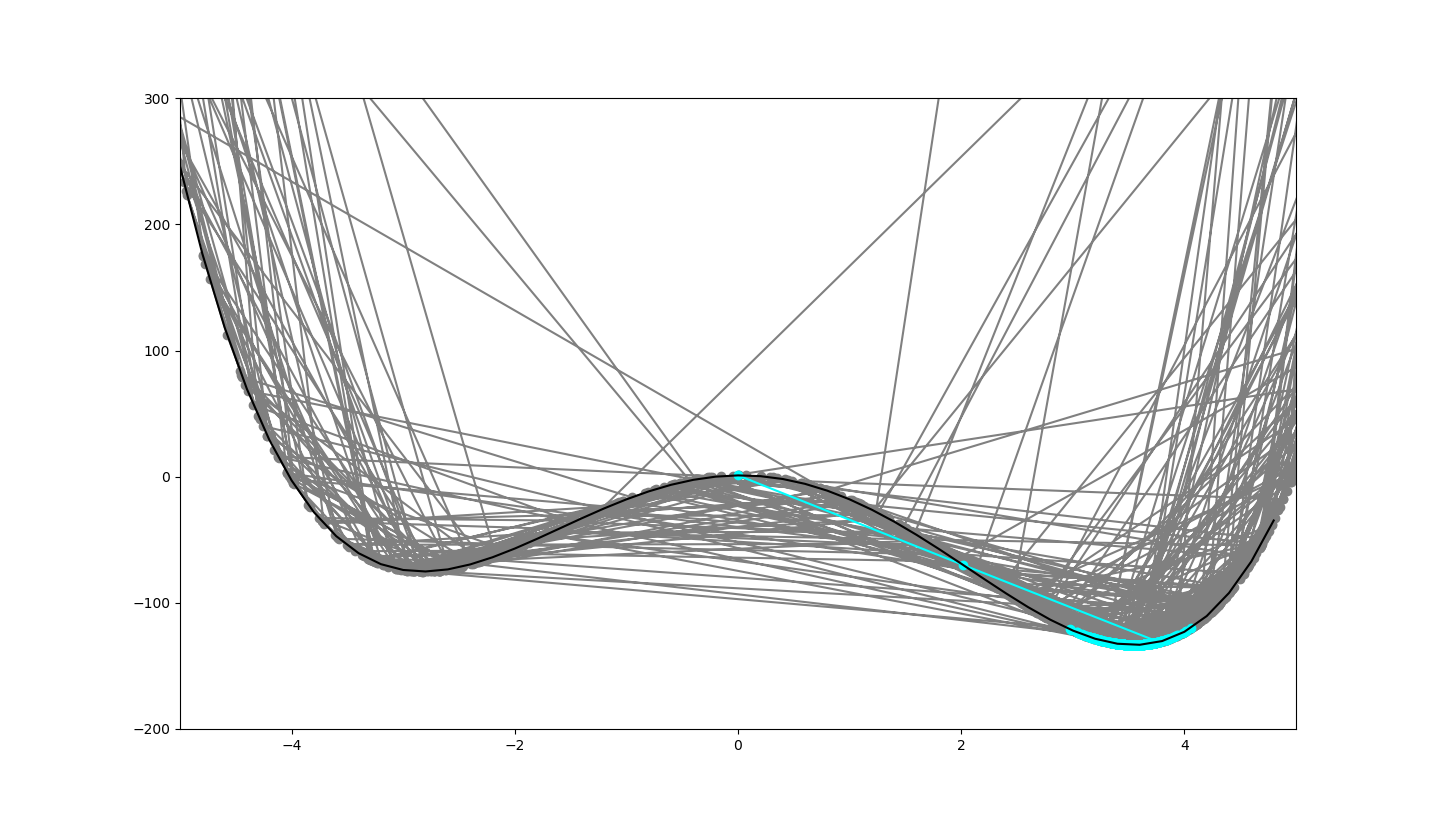
\includegraphics[width=0.45\textwidth]{recuitparpalliersF.png}
    \label{fig:a}%
    }%or more
    \subfigure[cas de la fonction g]{%
    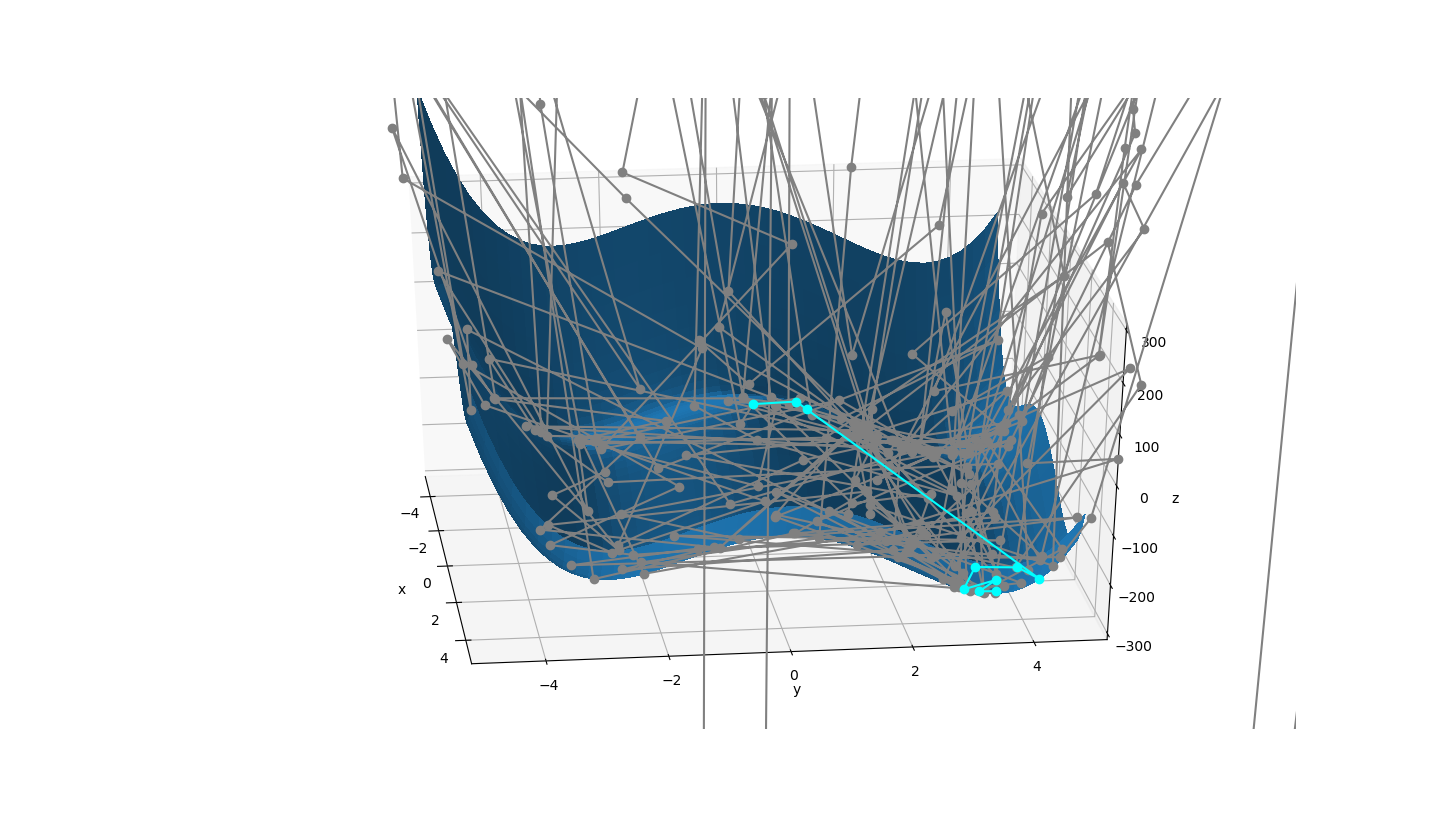
\includegraphics[width=0.45\textwidth]{ecuitparpalliers_G.png}
    \label{fig:b}%
  }%  
  \caption{Représentation du parcours de l'algorithme du recuit sans paliers en gris et avec paliers turquoise. Les conditions initiales sont choisies aléatoirement,  $k =15$, $k'=0.2$, et $t_max= 2000$}
  \label{fig:ab}
\end{figure}
D'après les figures ci-dessus il est claire que la différence majeur entre les deux versions est l'espace parcourut par l'algorithme. En effet en imposant l'exploration du voisinage avant de décider si on conserve ou pas une solution permet, d'augmenter la probabilité de conserver une mauvaise solutions si l'environnement est très variable ($\Delta E$ grand) et réciproquement si $\Delta E$ est petit. \\
On peut comparer l'efficacité des deux méthodes, ainsi pur la fonction $f$, en fixant $t_{max}=10000$, $k=10$;,$k'=0.5$ et pour des 21 conditions initiales choisies aléatoirement on obtient 71\% de succès pour la version sans exploration et 100\%, avec un paliers permettant d'estimer $\Delta E$ en 5 itérations. Pour ces simulations si nous calculons la distance parcourue en moyenne on trouve 232122 dans le cas sans paliers et seulement 1215 avec paliers, ce qui confirme nos observations.\\

\begin{minipage}{0.5\textwidth}
Le profil de l'acceptation entre les deux algorithme, permet de mettre en évidence leur mécanisme. Dans le premier  cas (bleu foncé) l'algorithme décroît exponentiellement tandis que dans le second cas la probabilité d'accepter une mauvaise réponse diminue d'abord très rapidement car dans une pende $\Delta E$ est faible puis augmente dès que  l'algorithme est dans un creux car alors $\Delta E$ est grand. Cette caractéristique permet à la nouvelle version de ressortir d'un minimum local.
\end{minipage} \hfill
\begin{minipage}{0.45\textwidth}
\begin{figure}[H]
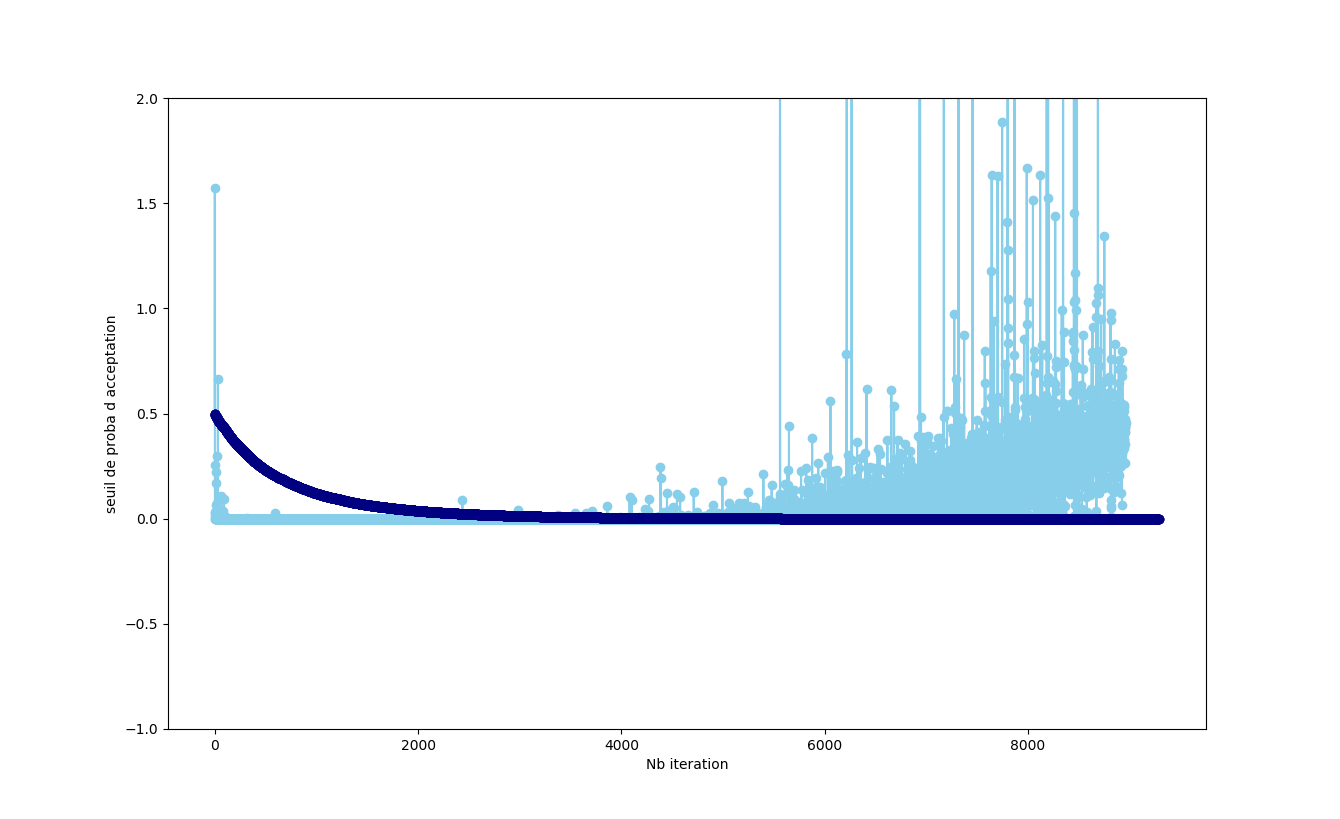
\includegraphics[width=1\textwidth]{PROBA_K.png}
\caption{Représentation de l'évolution de la probabilité d'acceptation d'une mauvaise solution, le première méthode est représentée en bleue foncé et la seconde en bleu clair. }
\label{Q2K}
\end{figure}
\end{minipage}


%% Pourquoi le paliers modifie l'éfficacité

\section{Le voyageur de commerce}
\begin{center}
\fcolorbox{black}{lightgray}{
\begin{minipage}{\linewidth}
\textbf{Principe :} \\
On utilise le principe du recuit simulé dans le cadre d'un problème d'optimisation discret. Considérant un certains nombre dans points dans un intervalle donné nous cherchons à réduire la distance permettant de relier tous ces points. Le paramètre à minimiser sera donc la distance Euclidienne entre les points. Nous nous servirons de l'algorithme précédemment construit. 

\end{minipage}}
\end{center}
\textbf{\color{brick}1.}
Pour générer un pays aléatoire nous utiliserons la fonction \verb|cities|.\\
\textbf{\color{brick}2.}
Pour calculer la distance Euclidienne entre les villes étant donné un trajet nous utiliserons la fonction \verb|distance|.\\
\textbf{\color{brick}3.}
Pour générer un voyage aléatoire étant donné un pays nous utliserons la fonction \verb|journey|.\\
\textbf{\color{brick}4.} Pour choisir le trajet optimal nous avons implémenter un algorithme de recuit simulé avec palier tel qu'il a été définit précédemment. La fonction est \verb|recuit_traveller|, elle prend en paramètre : un pays ,un trajet initial , une température, k , k', un nombre d'itérations maximal, un taux d'acceptation , un paliers (m), et un schéma de refroidissement. La fonction \verb|recuit\_traveller\_display| permet de générer à la compilation les graphiques des trajets et l'évolution de la distance. \\

\textbf{\color{brick}5.}
Nous pouvons oserver le comportement de l'algorithme les chamins proposés au cours des itération; pour cette simulation nous prendrons comme paramètre : un nombre de ville de 1 un carré de dimension 3, nous fixons $t_{max}=10$ ,$k=10$, $k'=0.5$, et $m=5$ (où m est la longeur du palier)

\begin{figure}[H]
  \centering
  \subfigure{%
    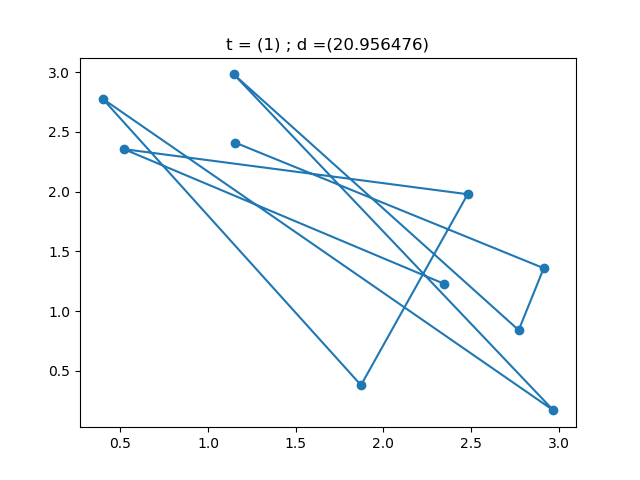
\includegraphics[width=0.45\textwidth]{voyage_0.png}
    }%or more
    \subfigure{%
    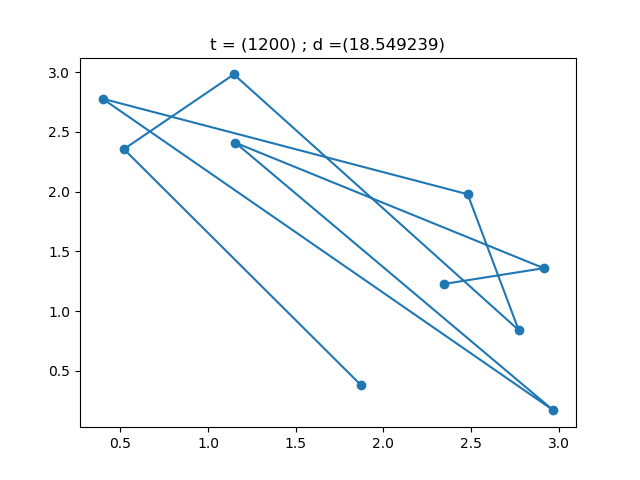
\includegraphics[width=0.45\textwidth]{voyage_1200.png}
 
  }\\ 
    \subfigure{%
    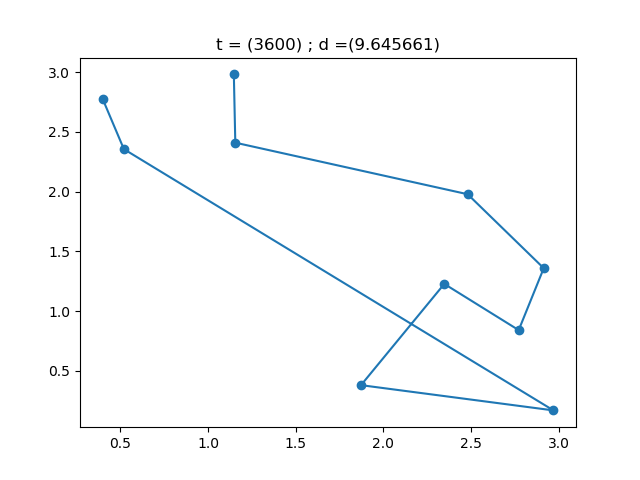
\includegraphics[width=0.45\textwidth]{voyage_3600.png}
    }%or more
    \subfigure{%
    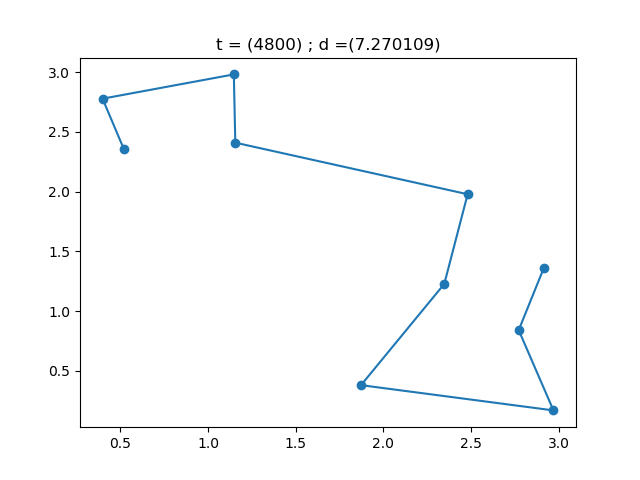
\includegraphics[width=0.45\textwidth]{voyage_4800.png}
 
  }\\ 

 
      \subfigure{%
    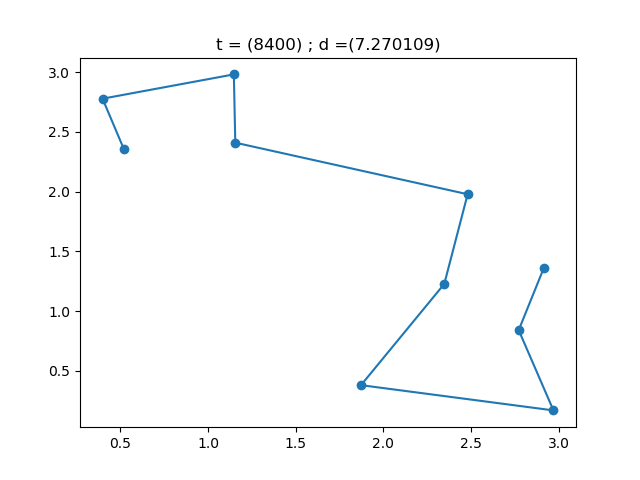
\includegraphics[width=0.45\textwidth]{voyage_8400.png}
    }%or more
    \subfigure{%
    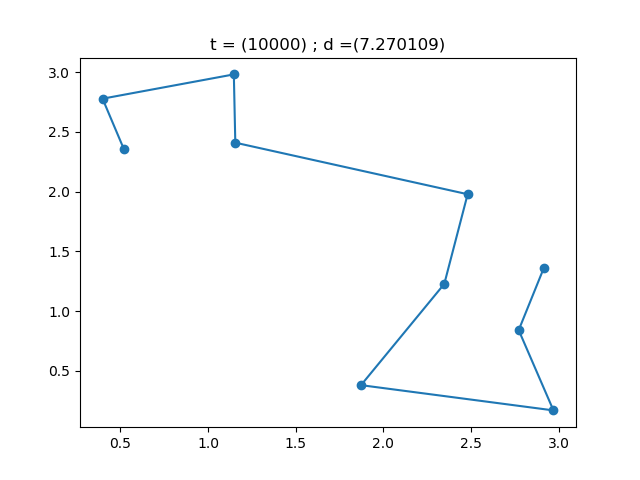
\includegraphics[width=0.45\textwidth]{voyage_10000.png}
 
  }\\
  \caption{Représentation de l'évolution des trajets au cours du temps.}
 \end{figure}


D'après la dynamique ci-dessus nous observons que l'algorithme du recuit simulé permet de réduire la distance parcourue, sans que nous ayons aucune certitude s'il parvient à trouver la distance minimale réel que nous ne connaissons pas. Cependant si pour le scénario précédent nous observons une diminution continue et la converge vers ce qui semble être le minimum global pour certaines simulations il peut arriver avec les mêmes paramètres d'obtenir en fin de simulation un résultat sous optimal par rapport à ceux précédemment trouvé. Le graphique représentant la distance par rapport au nombr de simulation permet de visualiser ce problème.


\begin{minipage}{0.5\textwidth}
D'après la dynamique ci-dessus nous observons que l'algorithme du recuit simulé permet de réduire la distance parcourue, sans que nous ayons aucune certitude s'il parvient à trouver la distance minimale réel que nous ne connaissons pas. Cependant si pour le scénario précédent nous observons une diminution continue et la converge vers ce qui semble être le minimum global pour certaines simulations il peut arriver avec les mêmes paramètres d'obtenir en fin de simulation un résultat sous optimal par rapport à ceux précédemment trouvé. Le graphique représentant la distance par rapport au nombr de simulation permet de visualiser ce problème. De plus remarquons qu'en début de simulation les solutions proposées sont très variables et oscillante, ce illustre la souplesse de l'algorithme.

\end{minipage} \hfill
\begin{minipage}{0.45\textwidth}
\begin{figure}[H]
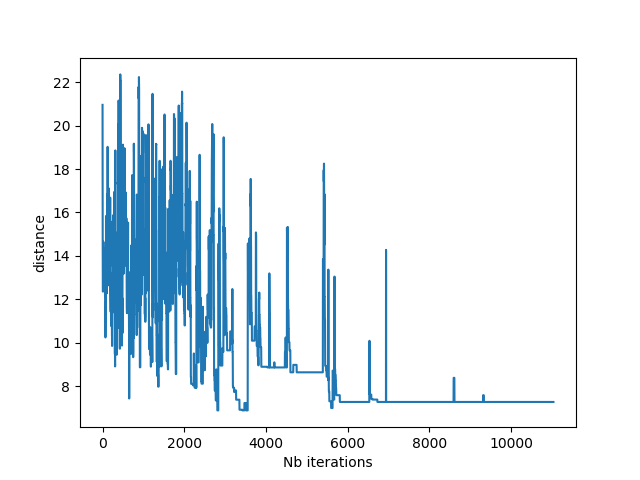
\includegraphics[width=1\textwidth]{distance_2.png}
\caption{Représentation l'évolution de la distance au cours des itérations. D'après ce graphique nous observons qu'un minimum trouvé dès 6000 itérations. Néanmoins l'apparition de pic témoigne que l'algorithme accepte parfois de 'mauvaise' solution avant de retomber vers le minimum précédemment calculé.  }
\label{Q2KP}
\end{figure}
\end{minipage}
\textbf{\color{brick}6.}  Analysons à présent les solutions pour différents schéma de refroidissement tels que :
 $T =\frac{1}{t}$,
  $T =\frac{1}{t^3}$,
 et $T =\frac{1}{log(t)}$.\\
 
\begin{figure}[H]
\centering
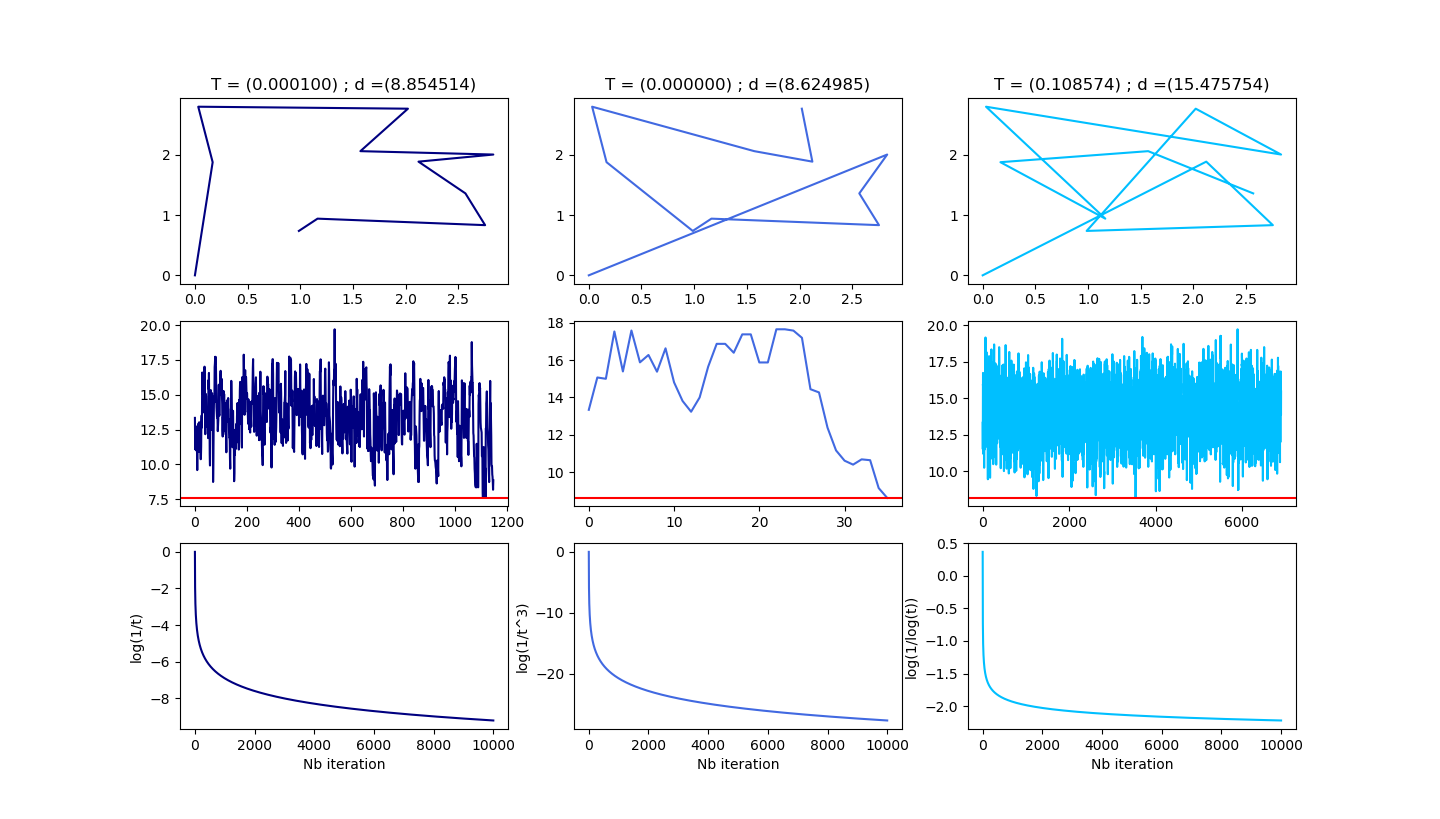
\includegraphics[width=1\textwidth]{schema_refroissement.png}
\caption{Représentation de l'évolution des solutions finales première ligne, de la distance au cours des itérations et le log de la température troisième ligne. La colonne 1 correspond au schéma de décroissance $\frac{1}{T}$, la seconde colonne à $\frac{1}{t^3}$ et la troisième à $\frac{1}{log(t)}$ .}
\label{refroidissement}
\end{figure}
 La figure \textbf{[\ref{refroidissement}]} met en évidence le compromis entre précision et temps de calcul. En effet on observe que plus  la décroissance de la température est rapide plus le temps de calcul est faible (ligne 2). Or si le schéma de refroidissement tel que $T = \frac{1}{t^3}$ est très rapide avec une convergence vers 30 itérations et une distance telle que $d\simeq 8.62$, la qualité de la solution retournée est moindre qu'avec le schéma de refroidissement $T  = \frac{1}{t}$ qui converge autour de 1200 itérations et propose une solution de $d\simeq8.854$. Ces observations sont confirmées par l'allure des solutions (ligne 1). Enfin  dans le cas où le refroidissement est équivalent à $T  = \frac{1}{log(t)}$, la diminution de la température est si lente qu'en 10000 itérations nous n'observons de minimisation de la distance parcourue.\\
Pour expliquer ces différentes observations nous pouvons rappeler que plus la température diminue rapidement plus on réduit rapidement la zone  et la probabilité d'acceptation de mauvaise solution. Si l'on cherche à être précis alors un schéma de décroissance tel que $T =\frac{1}{t^3}$ ne semble pas approprié puisque lorsque qu'un minimum est trouvé il semble difficile d'en ressortir, en revanche le temps de calcul est considérablement diminué. En revanche dans le cas où le schéma de décroissance est $T = \frac{1}{log(t)}$, alors d'une part l'algorithme accepte trop fréquemment de mauvaise solution et d'autre part il parcourt un voisinage trop éloigné du point courant, ceci implique qu'il ne parvient pas à se stabiliser.

\begin{figure}[H]

  \subfigure[Distance optimale]{%
    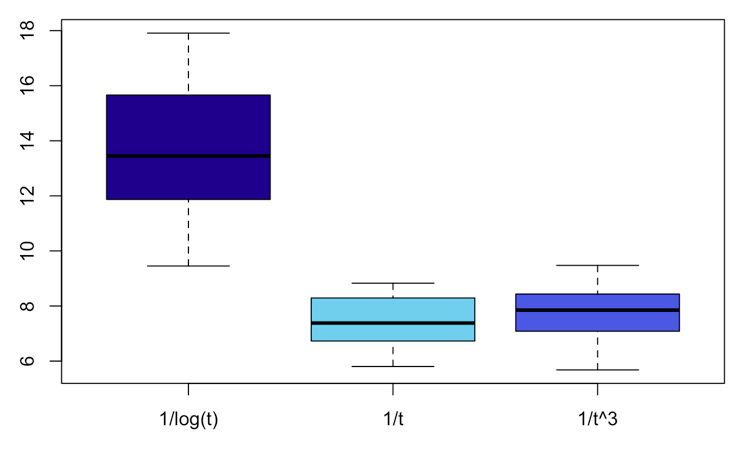
\includegraphics[width=0.45\textwidth]{dist_decroissance.png}
    \label{fig:aD}%
    }%or more
    \subfigure[Longueur du vecteur solutionsl ]{%
    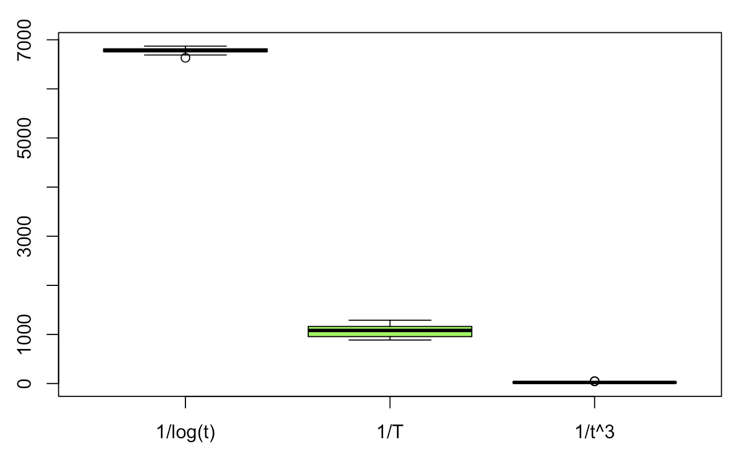
\includegraphics[width=0.45\textwidth]{dist_temps.png}
    \label{fig:bT}%
  }%  
  \caption{Représentation de la distance optimale \textbf{[\ref{fig:aD}]}  trouvée pour un pays de 10  villes modéliser par un carré de côté 3, $t_{max}=1000$, $k=10$, $k'=0.5$ et $m=5$  et représentation du temps nécessaire à la convergence  \textbf{[\ref{fig:bT}]} qui est équivalent à  la longueur du vecteur des solutions.}
  \label{fig:ab}
\end{figure}



 \end{document}